\documentclass[tikz,border=12pt]{standalone}
\usepackage[T1]{fontenc}
\usepackage{mathpazo}
\usepackage{amsmath,amssymb}
\usetikzlibrary{arrows.meta, positioning, calc, fit, patterns, decorations.pathreplacing}

\definecolor{stblue}{HTML}{7B97AD}
\definecolor{rwgold}{HTML}{B8995E}
\definecolor{sage}{HTML}{7A9A7E}
\definecolor{dkbrown}{HTML}{3D3530}
\definecolor{wmgray}{HTML}{7B7067}
\definecolor{cream}{HTML}{F9F6F0}
\definecolor{border}{HTML}{D4C9B8}
\definecolor{terracotta}{HTML}{C47A6A}
\definecolor{lavender}{HTML}{907EA0}

\begin{document}
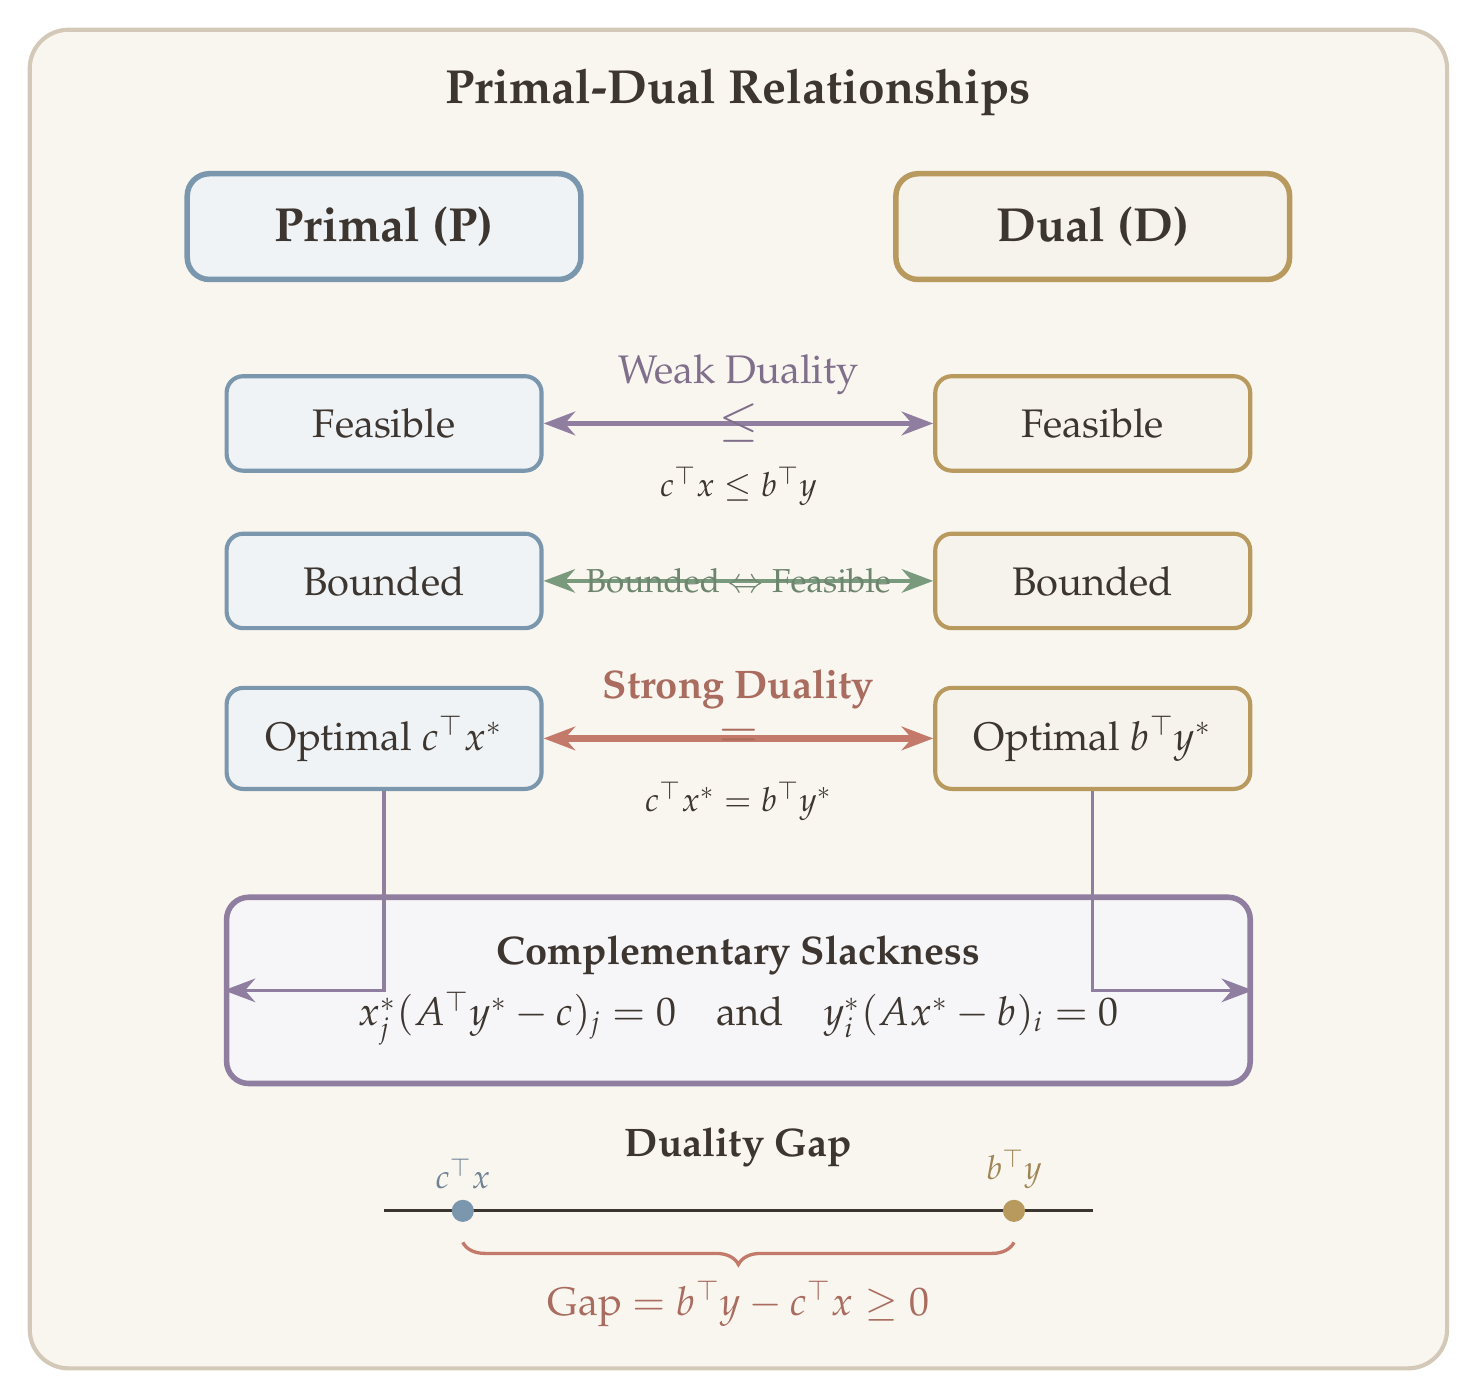
\begin{tikzpicture}[>={Stealth[length=4mm, width=3mm]}, line width=1.5pt,
  statusbox/.style={fill=#1!12, draw=#1, line width=1.5pt, rounded corners=6pt,
                    font=\Large, text=dkbrown, inner sep=10pt, minimum width=4.0cm,
                    minimum height=1.2cm, align=center}
]

% Background
\fill[cream, rounded corners=14pt] (-1,-7) rectangle (17,10);
\draw[border, line width=1.5pt, rounded corners=14pt] (-1,-7) rectangle (17,10);

% Title
\node[font=\LARGE\bfseries, text=dkbrown] at (8,9.2) {Primal-Dual Relationships};

% Column headers
\node[fill=stblue!12, draw=stblue, line width=2pt, rounded corners=8pt,
      font=\LARGE\bfseries, text=dkbrown, inner sep=12pt, minimum width=5.0cm]
  (primal-header) at (3.5,7.5) {Primal (P)};

\node[fill=rwgold!12, draw=rwgold, line width=2pt, rounded corners=8pt,
      font=\LARGE\bfseries, text=dkbrown, inner sep=12pt, minimum width=5.0cm]
  (dual-header) at (12.5,7.5) {Dual (D)};

% Primal column
\node[statusbox=stblue] (p-feas) at (3.5,5.0) {Feasible};
\node[statusbox=stblue] (p-bound) at (3.5,3.0) {Bounded};
\node[statusbox=stblue] (p-opt) at (3.5,1.0) {Optimal $c^\top x^*$};

% Dual column
\node[statusbox=rwgold] (d-feas) at (12.5,5.0) {Feasible};
\node[statusbox=rwgold] (d-bound) at (12.5,3.0) {Bounded};
\node[statusbox=rwgold] (d-opt) at (12.5,1.0) {Optimal $b^\top y^*$};

% Weak duality arrow
\draw[lavender, line width=2pt, <->] (p-feas.east) -- (d-feas.west)
  node[midway, above=6pt, font=\Large, text=lavender!80!dkbrown] {Weak Duality};
\node[font=\LARGE, text=lavender!80!dkbrown] at (8,5.0) {$\leq$};
\node[font=\large, text=dkbrown] at (8,4.2)
  {$c^\top x \leq b^\top y$};

% Boundedness relationship
\draw[sage, line width=1.5pt, <->] (p-bound.east) -- (d-bound.west);
\node[font=\large, text=sage!80!dkbrown] at (8,3.0) {Bounded $\Leftrightarrow$ Feasible};

% Strong duality
\draw[terracotta, line width=2.5pt, <->] (p-opt.east) -- (d-opt.west)
  node[midway, above=6pt, font=\Large\bfseries, text=terracotta!80!dkbrown] {Strong Duality};
\node[font=\LARGE\bfseries, text=terracotta!80!dkbrown] at (8,1.0) {$=$};
\node[font=\large, text=dkbrown] at (8,0.2)
  {$c^\top x^* = b^\top y^*$};

% Complementary slackness box at bottom
\node[fill=lavender!8, draw=lavender, line width=2pt, rounded corners=8pt,
      font=\Large, text=dkbrown, inner sep=14pt, minimum width=13cm, align=center]
  (cs) at (8,-2.2)
  {\textbf{Complementary Slackness}\\[4pt]
   $x_j^*(A^\top y^* - c)_j = 0 \quad \text{and} \quad y_i^*(Ax^* - b)_i = 0$};

% Arrows from optimal to CS
\draw[lavender, line width=1.2pt, ->] (p-opt.south) |- (cs.west);
\draw[lavender, line width=1.2pt, ->] (d-opt.south) |- (cs.east);

% Duality gap visualization
\node[font=\Large\bfseries, text=dkbrown] at (8,-4.2) {Duality Gap};
\draw[dkbrown, line width=1pt] (3.5,-5.0) -- (12.5,-5.0);
\fill[stblue] (4.5,-5.0) circle (4pt);
\node[font=\large, text=stblue!80!dkbrown, above=4pt] at (4.5,-5.0) {$c^\top x$};
\fill[rwgold] (11.5,-5.0) circle (4pt);
\node[font=\large, text=rwgold!80!dkbrown, above=4pt] at (11.5,-5.0) {$b^\top y$};
\draw[decorate, decoration={brace, amplitude=8pt, mirror}, terracotta, line width=1.2pt]
  (4.5,-5.4) -- (11.5,-5.4) node[midway, below=10pt, font=\Large, text=terracotta!80!dkbrown]
  {Gap $= b^\top y - c^\top x \geq 0$};

\end{tikzpicture}
\end{document}
